\documentclass[aps,%
12pt,%
final,%
oneside,
onecolumn,%
musixtex, %
superscriptaddress,%
centertags]{article} %%
\topmargin=-40pt
\textheight=650pt
\usepackage[english,russian]{babel}
\usepackage[utf8]{inputenc}
%всякие настройки по желанию%
\usepackage[colorlinks=true,linkcolor=blue,unicode=true]{hyperref}
\usepackage{euscript}
\usepackage{supertabular}
\usepackage[pdftex]{graphicx}
\usepackage{amsthm,amssymb, amsmath}
\usepackage{textcomp}
\usepackage[noend]{algorithmic}
\usepackage[ruled]{algorithm}
\selectlanguage{russian}

\begin{document}

\begin{titlepage}
\begin{center}
% Upper part of the page
\textbf{\Large САНКТ-ПЕТЕРБУРГСКИЙ \\ ГОСУДАРСТВЕННЫЙ УНИВЕРСИТЕТ} \\[1.0cm]
\textbf{\large Математико-Механический факультет} \\[0.2cm]
\textbf{\large Кафедра информационно аналитических систем}\\[3.5cm]

% Title
\textbf{\LARGE Суммаризация групп в социальных сетях}\\[1.0cm]
\textbf{\Large Дипломная работа студента 645 группы} \\[0.2cm]
\textbf{\Large Чурикова Никиты Сергеевича} \\[3.5cm]

%supervisor
\begin{flushright} \large
\emph{Научный руководитель:} \\
к.ф. - м.н., доцент \textsc{Графеева Н. Г.}
\end{flushright}
 \begin{flushright} \large
\emph{Рецензент:} \\
Руководитель департамента вычислительной биологии \textsc{Яковлев П. А.}
\end{flushright}
\begin{flushright} \large
\emph{Заведующий кафедрой:} \\
к.ф. - м.н., доцент \textsc{Михайлова Е. Г.}
\end{flushright}
\vfill

% Bottom of the page
{\large {Санкт-Петербург}} \par
{\large {2019 г.}}
\end{center}
\end{titlepage}

% Table of contents
\tableofcontents

\section{Аннотация}
Одной из задач обработки естественного языка является задача суммаризации текста.
Ее целью является уменьшение размера исходного текста без потери ключевой информации.
В данной работе мы решаем схожую проблему, но для информационных ресурсов в социальных сетях.
В частности, необходимо рассмотреть задачу суммаризации текстов и картинок, поскольку
это два основных источника информации. В тексте мы приводим численное обоснование
выбранных методов, а также приводим оценку нашей суммаризации людьми.

\section{Введение}
В современном мире создается все больше и больше информации, которую мы можем потреблять.
Новости, статьи, юмор постоянно меняются и создаются людьми. При таком потоке информации
появляется потребность в инструментах, способных давать как можно больше информации
с минимальными потерями.

При чтении новостей люди, как правило, не идут дальше новостных заголовков \cite{jaysondemers2016},
для популярных технических статей создают краткие описания описывающие их достижения
и основные моменты \cite{tldr_arxiv2019, articleessence2019}, а визуальный контент нередко подчиняется единому шаблону.

В данной работе мы показываем, как используя современные достижения в области анализа
данных можно извлекать полезную информацию из новостных ресурсов в социальной сети вконтакте \cite{vk2019},
приводим оценки людей нашей системы и приводим сравнение с наивными решениями.

\subsection{Постановка задачи}
Мы поставили перед собой задачу создать систему, которой бы можно было передавать ссылку на новостной ресурс в социальной сети вконтакте, а на выходе получать его краткое описание. В рамках работы мы ограничились новостными ресурсами с высоким содержанием текста.

С алгоритмической точки зрения, задача суммаризации новостного ресурса была рассмотрена нами как две подзадачи:
\begin{enumerate}
  \item Извлечение ключевых слов, присущих данному источнику информации;
  \item Сжатие новостей, используя автоматическое создание заголовков.
\end{enumerate}

Через извлечение данной информации мы хотим добиться эффекта "чтения по диагонали".

Для оценки качества наших алгоритмов, мы воспользовались открытыми датасетами для суммаризации текстов, а также проводили оценку качества людьми.
\subsection{Обзор литературы}
Задача сжатия текста с малой потерей смысла и сохранением возможности его прочтения
имеет название задачи \textit{суммаризации}. При этом, есть два концептуальных подхода к решению:
экстрактивный, когда для создания краткого содержания извлекаются целые куски текста вплоть до предложений,
и абстрактивная, где в кратком содержании могут быть слова, которых не было в исходном тексте.

В частности, при исследовании абстрактивной генерации заголовков, мы отталкивались от статьи Вконтакте, посвященной данной проблеме \cite{gavrilov2018self}. Ими предлагается применять нейронные сети с архитектурой Transformer и предобработкой Byte pair encoding (BPE) \cite{DBLP:journals/corr/SennrichHB15}. Однако в задаче абстрактивной генерации заголовков существуют дебаты на тему того, что использовать в качестве входа модели. Поскольку долгое время SOTA были модели с архитектурой encoder decoder, то было невозможно использовать длинные входные последовательности. Потому авторы статьи \cite{Putra2018IncorporatingTS} исследуют различные подходы по предварительному извлечению "Topic sentence", которое нейронная сеть должна дальше обработать. Это предложение, как говорят авторы, в идеальном случае, должна отвечать на 5W1H. Но достаточно ответов на "что, кто, когда".

Для экстрактивной суммаризации чаще всего используют алгоритм TextRank \cite{TextrankOriginal}. Идея
% TODO: Add more desctiption


\subsection{Полученные результаты}
Что является результатом работы (будет веб сервис, куда можно закинуть ссылку на группу),
как оценивали качество (продолжить результаты работы алгоритмов толокерам), а также
оценка качества по автоматизированным метрикам, и как они коррелируют с оценками людей.
Сравниться с бэйзлайном.

\section{Алгоритмы, использованные в работе}
Нами были использованы как классические подходы, так и новые, основанные на нейронных сетях.
В следующих секциях мы опишем их основные принципы, а также приведем ссылки на их реализации.

\subsection{Суммаризация текста}
Для суммаризации текста мы воспользовались алгоритмом экстрактивной суммаризации
основанном на TextRank \cite{DBLP:journals/corr/BarriosLAW16, rehurek_lrec, TextrankOriginal},
и моделью трансформера \cite{DBLP:journals/corr/VaswaniSPUJGKP17}, обученной на
датасете РИА новостей \cite{gavrilov2018self}.
Для предобработки данных модели трансформера мы использовали byte
pair encoding \cite{DBLP:journals/corr/SennrichHB15}.
Помимо этого мы извлекали первое предложение из новости.
Для TextRank и извлечения первого предложения не требуется обучающая выборка, что
делает их очень удобными в использовании. При этом, исследования показывают, что
в задаче генерации заголовков, первое предложение в новости --
это очень сильный бэйзлаин \cite{gavrilov2018self},
который трудно побить как экстрактивной, так и абстрактивной суммаризацией.

\subsubsection{TextRank}

TextRank является является адаптацией идеи алгоритма PageRank \cite{Page98thepagerank} с задачи рекомендации страниц в интернете на задачу рекомендации лучшего предложения или набора слов в тексте. Сам алгоритм состоит в том, что мы текст превращаем в граф, где узлы -- это предложения, а для каждого ребра подсчитывается вес, где вес определяется по количеству совпавших слов в двух предложениях.

Таким образом, получается, что можно выбрать предложение с самыми тяжелыми ребрами в качестве предложения, которое описывало бы исходный текст.

\begin{figure}[ht]
\begin{center}

\scalebox{0.4}{
   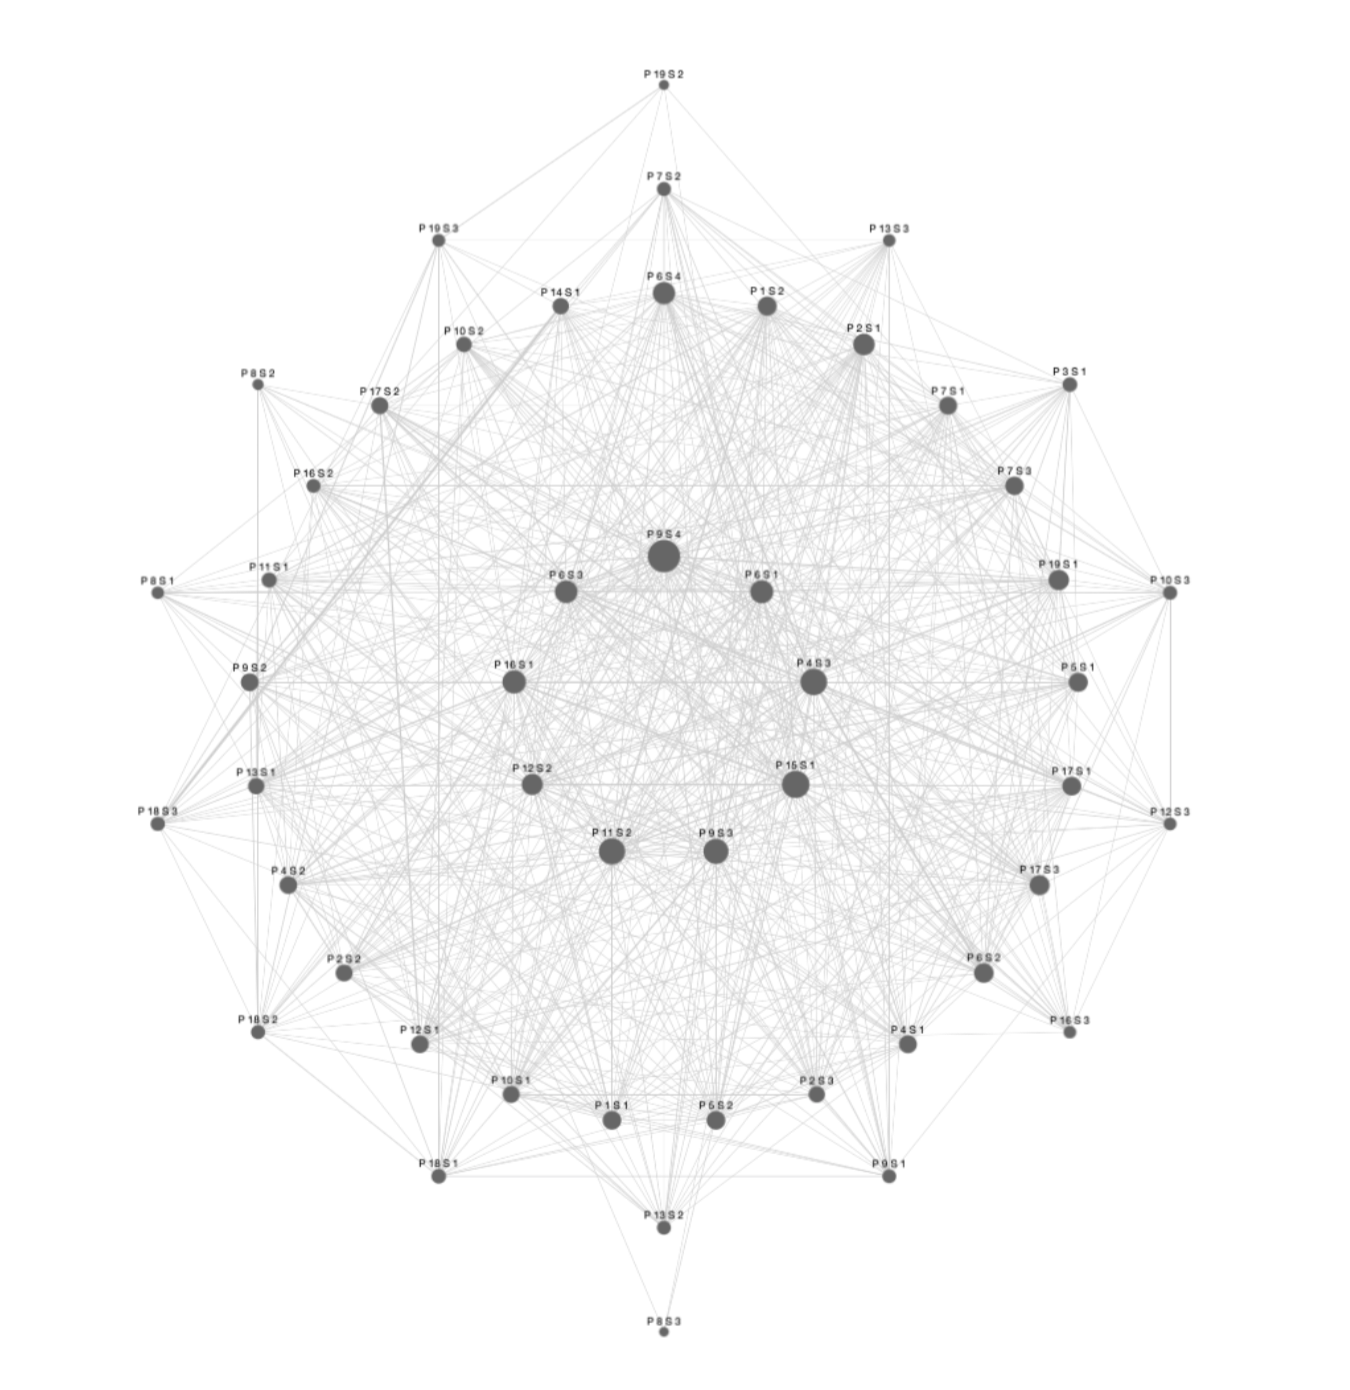
\includegraphics{images/text_rank_example_graph.png}
}

\caption{
\label{text_rank_example_graph}
        Пример результирующего графа textrank.}
\end {center}
\end {figure}

\subsubsection{Byte pair encoding}

\subsubsection{Transformer network}

% \subsection{Суммаризация изображений}
% Для суммаризации изображений мы реализовали алгоритм,
% описанный в статье \cite{DBLP:conf/icsipa/SharmaKASK15}.
% Основная идея состоит в том, что из изображений извлекаются
% признаки, инвариантные к поворотам \cite{Lowe:2004:DIF:993451.996342},
% эти признаки кластеризуют
% используя k-means \cite{Arthur:2007:KAC:1283383.1283494} и индексы кластеров
% используют как признаки для латентного размещения
% Дирихле \cite{Blei:2003:LDA:944919.944937, rehurek_lrec}.
%
% Помимо этого, мы попробовали
% на нашей задаче обучению метрике между изображениями
% \cite{DBLP:journals/corr/abs-1803-11095, DBLP:journals/corr/abs-1810-06951}.

\subsection{Оценки качества}
Для оценки качества текстовых моделей мы использовали метрику ROUGE-L F1 \cite{Lin:2004},
при этом мы считали ее на датасете РИА новостей \cite{gavrilov2018self}.

Помимо этого, как для текстовых данных, так и для изображений, мы  использовали
Яндекс.Толоку \cite{yandex_toloka_2019}, чтобы привлечь людей к оценке качества наших результатов.

\section{Эксперименты}
Для обучения моделей были использованы 8 Tesla K80.

\section{Заключение}
На февраль 2019:

В данной работе мы ожидаем показать, что предложенные нами решения не хуже,
а даже лучше предложенных бэйзлайнов как по автоматическим оценкам, так и по оценкам
людей. Мы также представим код и ссылку на сервис, куда можно отправить ссылку на
интересующую группу и оценить получившийся результат.

\section{Литература}

\bibliographystyle{gost780s}
\bibliography{test}

\end{document}
